\documentclass{article}

\usepackage[UTF8]{ctex}
\usepackage{placeins}
\usepackage{graphicx}
\usepackage{listings}
\usepackage{xcolor} % 添加 xcolor 宏包
\lstset{ %
language=matlab,                % choose the language of the code
basicstyle=\footnotesize,       % the size of the fonts that are used for the code
numbers=left,                   % where to put the line-numbers
numberstyle=\footnotesize,      % the size of the fonts that are used for the line-numbers
stepnumber=1,                   % the step between two line-numbers. If it is 1 each line will be numbered
numbersep=5pt,                  % how far the line-numbers are from the code
backgroundcolor=\color{white},  % choose the background color. You must add \usepackage{color}
showspaces=false,               % show spaces adding particular underscores
showstringspaces=false,         % underline spaces within strings
showtabs=false,                 % show tabs within strings adding particular underscores
frame=single,           % adds a frame around the code
tabsize=2,          % sets default tabsize to 2 spaces
captionpos=b,           % sets the caption-position to bottom
breaklines=true,        % sets automatic line breaking
breakatwhitespace=false,    % sets if automatic breaks should only happen at whitespace
escapeinside={\%*}{*)}          % if you want to add a comment within your code
}
\title{hw06\_MATLAB}
\author{3220103167 缪晨轩}
\date{\zhdate{2024/4/9}}

\begin{document}
    \maketitle
    \section*{24(1)}
        \begin{lstlisting}[caption={题24(1) MATLAB代码}, label={lst:matlab}]
            n = -3:100; % 选择一个足够大的范围以确保序列趋于零
            x1 = (1/2).^n .* (n >= -3); % 定义序列x1(n)
            omega = -pi:0.01:pi; % 选择频率范围

            % 计算DTFT
            X1 = sum(x1 .* exp(-1i * omega' * n), 2);

            % 绘制幅度谱和相位谱
            subplot(2,1,1);
            plot(omega, abs(X1));
            xlabel('Frequency (\omega)');
            ylabel('|X_1(e^{j\omega})|');
            title('Magnitude Spectrum');

            subplot(2,1,2);
            plot(omega, angle(X1));
            xlabel('Frequency (\omega)');
            ylabel('Phase (radians)');
            title('Phase Spectrum');

        \end{lstlisting}
        Answer: 
            \begin{figure}[h]
                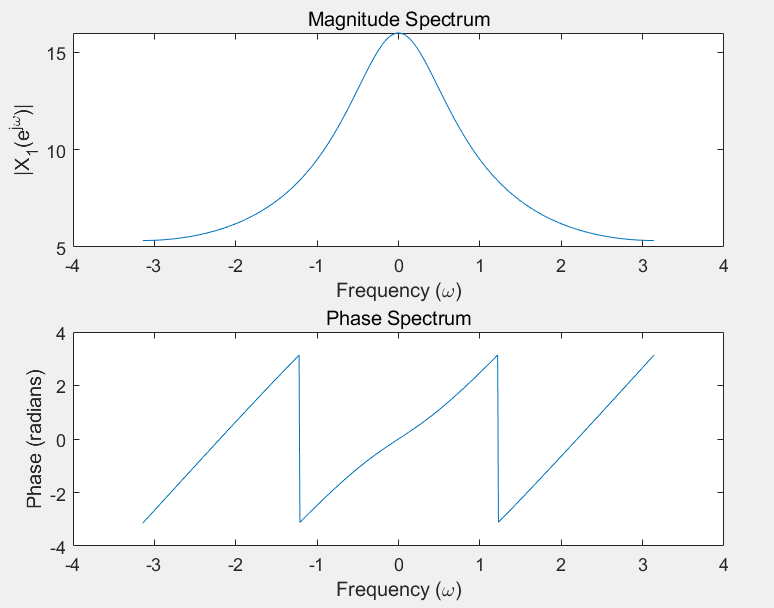
\includegraphics{24_1.png}
            \end{figure}
            \FloatBarrier
    \section*{24(2)}
        \begin{lstlisting}[caption={题24(2) MATLAB代码}, label={lst:matlab}]
            n = 0:100; % 选择一个足够大的范围以确保序列趋于零
            a = 0.5; % a的值(可以根据需要调整)
            omega_0 = pi/4; % \omega_0的值(可以根据需要调整)
            x2 = a.^n .* sin(n * omega_0); % 定义序列x2(n)
            omega = -pi:0.01:pi; % 选择频率范围

            % 计算DTFT
            X2 = sum(x2 .* exp(-1i * omega' * n), 2);

            % 绘制幅度谱和相位谱
            subplot(2,1,1);
            plot(omega, abs(X2));
            xlabel('Frequency (\omega)');
            ylabel('|X_2(e^{j\omega})|');
            title('Magnitude Spectrum');

            subplot(2,1,2);
            plot(omega, angle(X2));
            xlabel('Frequency (\omega)');
            ylabel('Phase (radians)');
            title('Phase Spectrum');

        \end{lstlisting}
        Answer: 
            \begin{figure}[h]
                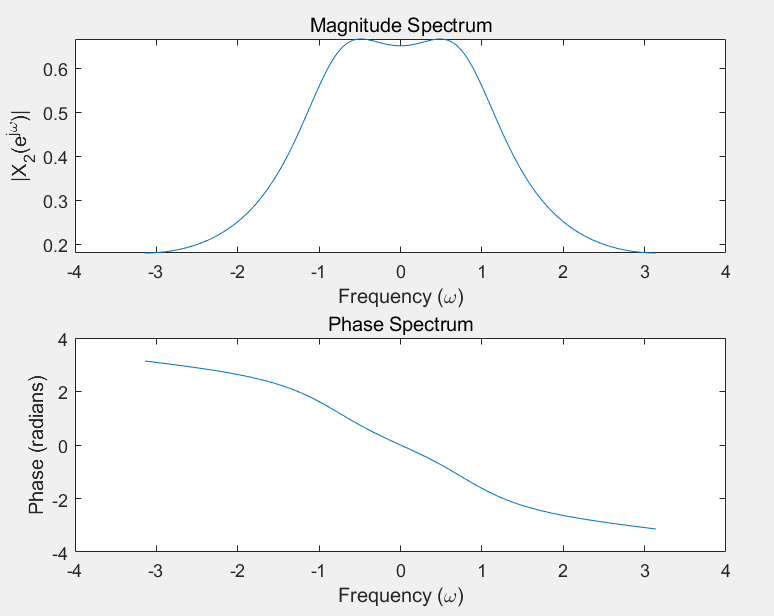
\includegraphics{24_2.png}
            \end{figure}
            \FloatBarrier
    \section*{24(3)}
        \begin{lstlisting}[caption={题24(3) MATLAB代码}, label={lst:matlab}]
            k = 0:100; % 选择一个足够大的范围以确保序列趋于零
            x3 = (1/2).^(2*k); % 定义序列x3(k)
            omega = -pi:0.01:pi; % 选择频率范围

            % 计算DTFT
            X3 = sum(x3 .* exp(-1i * 2 * omega' * k), 2);

            % 绘制幅度谱和相位谱
            subplot(2,1,1);
            plot(omega, abs(X3));
            xlabel('Frequency (\omega)');
            ylabel('|X_3(e^{j\omega})|');
            title('Magnitude Spectrum');

            subplot(2,1,2);
            plot(omega, angle(X3));
            xlabel('Frequency (\omega)');
            ylabel('Phase (radians)');
            title('Phase Spectrum');

        \end{lstlisting}
        Answer:
            \begin{figure}[h]
                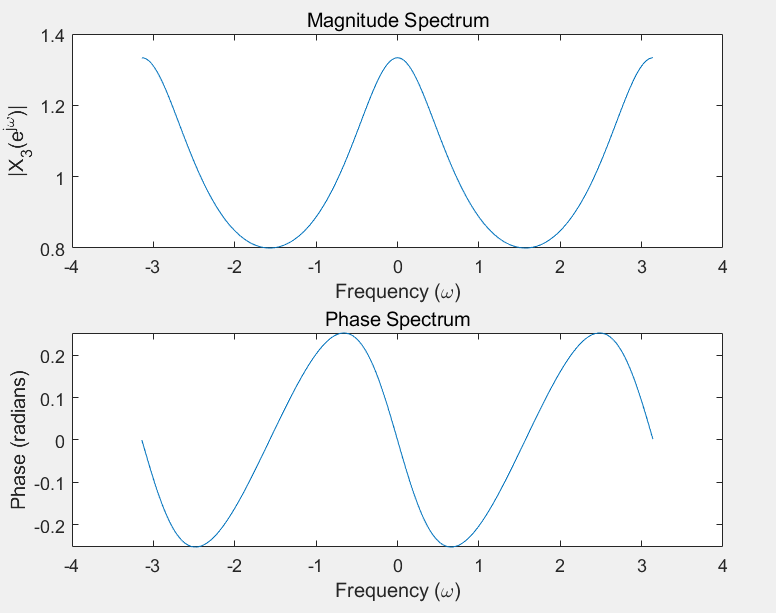
\includegraphics{24_3.png}
            \end{figure}
            \FloatBarrier
    
    \section*{25}
        \begin{lstlisting}[caption={题25 MATLAB代码}, label={lst:matlab}]
            % 定义采样频率和采样间隔
            fs = 1000; % 采样频率为1kHz
            Ts = 1/fs; % 采样间隔

            % 定义周期连续信号的参数
            A = 1;
            B = 2;

            % 定义离散时间信号的长度
            N = 1000; % 采样点数

            % 计算离散时间信号的值
            n = 0:N-1;
            xa = A*cos(200*pi*n*Ts) + B*cos(500*pi*n*Ts);

            % 计算离散傅里叶变换
            X = fft(xa);

            % 绘制离散傅里叶变换结果
            f = linspace(0, fs*(N-1)/N, N); % 频率轴
            stem(f, abs(X)); % 绘制幅度谱
            xlabel('频率 (Hz)');
            ylabel('幅度');
            title('DFS幅度谱');

        \end{lstlisting}
        Answer:
            \begin{figure}[h]
                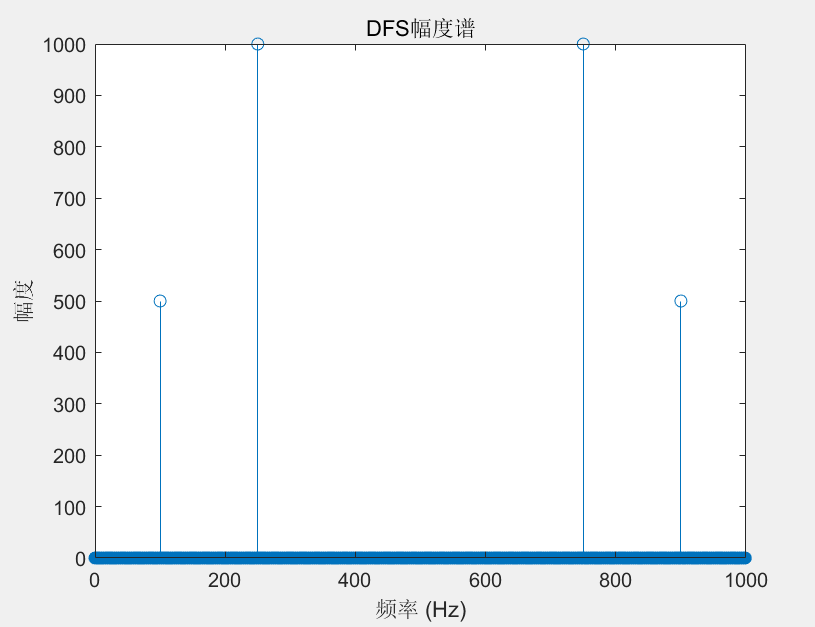
\includegraphics{25.png}
            \end{figure}
            \FloatBarrier
\end{document}